
By comparing observational data $\dv$ with a theoretical model $\fv$, one can address the following:
\begin{enumerate}
\item Determine whether a given theoretical model $\fv$ can explain the observational data.
\item Assuming that a theoretical model $\fv$ is correct, determine or estimate the parameters $\thetav$ included in that model based on the data $\dv$ ({\bf parameter estimation}).
\item When multiple models exist, determine which model better explains the observations $\dv$ ({\bf model selection}).
\end{enumerate}

Since model selection is considerably more involved, here we focus on parameter estimation.

As an example, let us consider the comparison between radial velocity observational data and a theoretical model. In this case, $\dv$ can be regarded as a vector consisting of the radial velocity data series, with each element $d_i$ associated with the corresponding time $t_i$, making it comparable to the theoretical model. The theoretical model is given by Eq.~(\ref{eq:vrsatarefinal}). The parameter vector is $\thetav = (V_\mathrm{sys}, K_\star, e, \omega, T_0, P)$.

\begin{itembox}{Radial velocity raw data $\dv$}
\footnotesize
\color{gray}
See \href{https://github.com/HajimeKawahara/class25}{https://github.com/HajimeKawahara/class25}
.
\end{itembox}

\section{Point estimation and optimization}

Parameter estimation that selects a single parameter vector $\thetav$ for a model $\fv(\thetav)$ by comparing it with data $\dv$ is called \underline{point estimation}. If the data contained no errors at all, we would simply need to find $\thetav$ such that
\begin{align}
\dv - \fv(\thetav) = \boldsymbol{0} .
\end{align}
However, in practice, observational data contain errors, and such a $\thetav$ usually cannot be found. Instead, we can write
\begin{align}
\dv = \fv(\thetav^\ast) + \epsilonv ,
\end{align}
which implies that the model $\fv$ is correct, that a “true” parameter $\thetav^\ast$ exists, and that the residual vector $\epsilonv$ originates solely from observational errors. To formulate the theory in a way that incorporates observational errors, we need a probabilistic model that generates these errors. For example, if $\epsilonv$ follows an independent zero-mean normal distribution,
\begin{align}
\epsilon_i \sim \mathcal{N}(0,\sigma) ,
\end{align}
we can write more compactly that the physical model $\fv(\thetav^\ast)$ is the mean of the probabilistic model:
\begin{align}
d_i \sim \mathcal{N} (f_i(\thetav^\ast), \sigma) .
\end{align}

From this discussion, it becomes clear that when we speak of comparing observational data with a theoretical model, the theoretical model must include not only $\fv$ but also a probabilistic model. Schematically,
\begin{itembox}{Empirically testable theoretical model}
Testable theory = Physical/Chemical model $+$ Probabilistic model
\end{itembox}

In practice, theoretical astronomy often overemphasizes the physical/chemical model while neglecting the probabilistic model, whereas observational astronomy tends to fix the physical/chemical model. Constructing probabilistic models has historically been computationally demanding and thus difficult to handle until recently. However, advances in computing power and Bayesian statistical methods now allow us to tackle this issue.

Returning to point estimation: although observational errors are often correlated, we leave their treatment to Gaussian process modeling and for now assume independent errors. Further, suppose these errors are Gaussian with the same $\sigma$ for all data points. In this case, the probability that a model $\fv(\thetav)$ with parameter vector $\thetav$ generates $\dv$ is
\begin{align}
p(\dv|\thetav) &= \prod_{i=1}^N \mathcal{N} (f_i(\thetav), \sigma ) \\
&\propto \exp{\left( - \dfrac{\sum_{i=1}^N (f_i(\thetav) - d_i)^2 }{2 \sigma^2}\right)} .
\end{align}
This is the likelihood function. The method that adopts as the point estimate the $\thetav$ that maximizes the likelihood is called the maximum likelihood method. In this case, we solve the optimization problem
\begin{align}
\thetav^\ast &= \mathrm{minimize}_{\thetav} \, L_2(\thetav) \\
L_2(\thetav) &= \sum_{i=1}^N (f_i(\thetav) - d_i)^2 ,
\end{align}
which is exactly the least squares method. In other words, the least squares method coincides with maximum likelihood estimation under the assumption of independent Gaussian errors.

A relaxed version of the assumptions behind least squares point estimation is $\chi^2$ minimization. Assuming that the error $\sigma_i$ of each data point is known,
\begin{align}
p(\dv|\thetav) &\propto \exp{\left( - \sum_{i=1}^N \dfrac{ (f_i(\thetav) - d_i)^2 }{2 \sigma_i^2}\right)} ,
\end{align}
we then solve the optimization problem
\begin{align}
\thetav^\ast &= \mathrm{minimize}_{\thetav} \, \chi^2(\thetav) \\
\chi^2(\thetav) &= \sum_{i=1}^N \dfrac{ (f_i(\thetav) - d_i)^2 }{2 \sigma_i^2} .
\end{align}


\section{Optimization problems and automatic differentiation}

From the above discussion, it is clear that the practical task of point estimation is an optimization problem. To solve nonlinear model optimization problems, there are many methods: Newton's method as a second-order optimization discussed earlier, its extensions such as quasi-Newton methods, the Marquardt method implemented by many researchers while studying Numerical Recipes, or derivative-free methods like the Nelder–Mead method, also known as the amoeba method.

Here, however, we focus on first-order optimization using automatic differentiation. This is because when the number of parameters is large, second-order optimization becomes limited by the computation of the Hessian. For this reason, machine learning models such as neural networks often rely on first-order optimization. The basic first-order method is gradient descent,
\begin{align}
\thetav^{(k)} &= \thetav^{(k-1)} - \gamma \frac{\partial}{\partial \thetav} f(\thetav) ,
\end{align}
which proceeds by descending the steepest slope. Since pure gradient descent often overshoots, various momentum terms are added to improve convergence. A representative method is ADAM \cite{kingma2015adam}, though we do not go into its algorithmic details here.

\begin{figure}[htb]
\begin{center}
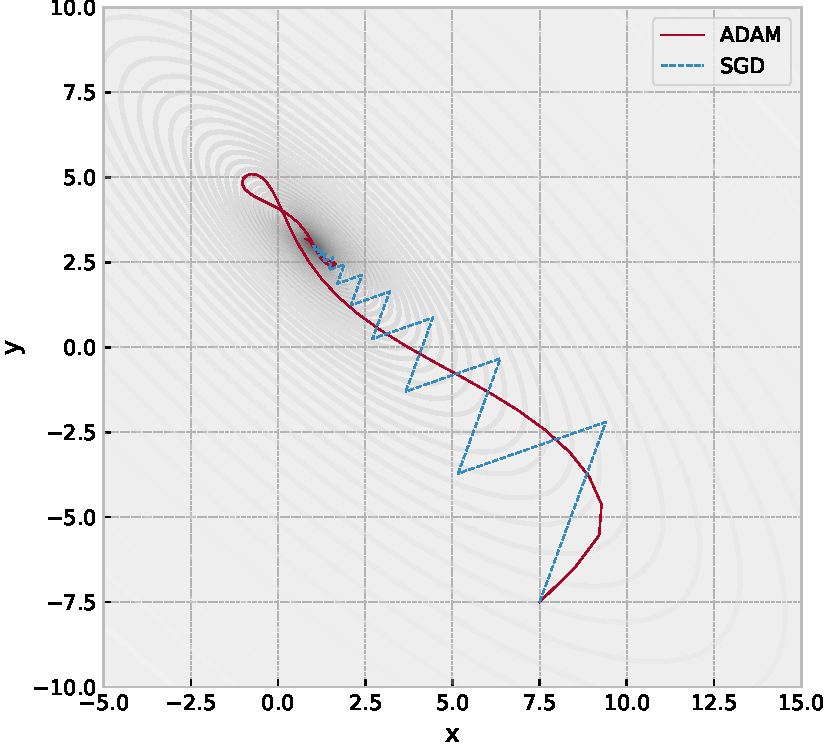
\includegraphics[width=\linewidth]{fig/opt1.pdf}
\caption{Example of first-order optimization.\label{fig:opt1}}
\end{center}
\end{figure}

First-order optimization requires derivatives of the model with respect to its parameters. Broadly speaking, there are four ways to compute derivatives numerically. The first is to perform differentiation by hand (manual differentiation) and code the results. This quickly becomes impractical as models grow more complex, and it also hinders flexible improvements to the model. The second approach is to use symbolic differentiation with tools such as Mathematica to obtain derivative expressions instead of differentiating by hand. However, as anyone who has used such tools knows, complex models generate enormous expressions, which again limits flexibility. The third approach is numerical differentiation, but for complex models, numerical errors can accumulate easily.

For this reason, machine learning and related fields often use automatic differentiation, as implemented in {\sf JAX/tensorflow/pytorch} etc. A model that can be coded is usually composed of additions, subtractions, multiplications, and divisions of functions whose derivatives are known (here we call these elementary functions). Automatic differentiation extends each elementary function
\begin{align}
x:\to f(x)
\end{align}
so that it outputs both the function value and its derivative. Operations are then defined so that the usual addition, multiplication, and division rules for derivatives hold.

In {\sf JAX}, automatic differentiation is implemented using the Jacobian–Vector Product (JVP). As an introduction, however, we explain automatic differentiation using dual numbers, which provides a simpler explanation.

A dual number, $z \in k[\epsilon]/\langle \epsilon^2\rangle$\footnote{This denotes a quotient ring of a polynomial ring.}, is defined for $a, b \in \mathbb{R}$ as
\begin{align}
z &= a + b \epsilon \\
\epsilon^2 &= 0 .
\end{align}
One may think of this as analogous to complex numbers, except that while $i^2 = -1$, here $\epsilon^2 = 0$. By extending a variable $x$ with the real part $a = x$ and the non-real part $b = x^\prime$, for $z = f + f^\prime \epsilon, w = g + g^\prime \epsilon$, addition, multiplication, and division are defined as
\begin{align}
\label{eq:add_ad_dual}
z + w &= (f + g) + (f^\prime + g^\prime) \epsilon \\
\label{eq:mul_ad_dual}
z w &= f g + (f^\prime g + f g^\prime) \epsilon \\
z/w &= \frac{f}{g} + \frac{f^\prime g - f g^\prime}{g^2} \epsilon .
\end{align}
This shows that the real part follows the usual arithmetic, while the non-real part follows the sum, product, and quotient rules of differentiation.

To realize the chain rule, a function $x:\to F(x)$ is extended as
\begin{align}
\label{eq:funcdual}
x+x^\prime \epsilon: \to F(x) + F^\prime(x) x^\prime \epsilon .
\end{align}
Here, $F(x)$ denotes the original function, while the extension with dual numbers is denoted $\hat{F}(x+x^\prime \epsilon)$. Thus, Eq.~(\ref{eq:funcdual}) can be written as
\begin{align}
\label{eq:chain_ad}
\hat{F}(x+x^\prime \epsilon) = F(x) + F^\prime(x) x^\prime \epsilon .
\end{align}
For a composite function $G(F(x))$, the extension becomes
\begin{align}
\hat{G}(\hat{F}(x+x^\prime \epsilon)) &= \hat{G}(F(x) + F^\prime(x) x^\prime \epsilon) \\
&= G(F(x)) + G^\prime(F(x)) F^\prime(x) x^\prime \epsilon ,
\end{align}
where the real part corresponds to the usual composition $G(F(x))$, and the non-real part reproduces the chain rule $G^\prime(F(x)) F^\prime(x) x^\prime = \dfrac{d G}{d F} \dfrac{d F}{d x} x^\prime$. \\


\subsection*{Minimal implementation of automatic differentiation}

Let us now implement a small version of automatic differentiation in Python. The problem we want to solve is to compute the derivative $F^\prime(1)$ of
\begin{align}
\label{eq:sample_func}
F(x) = \log{(\cos{x} \sin{x})} + \sin{x}
\end{align}
at $x=1$. Furthermore, we also want to find the derivative $G^\prime(1)$ of the composite function
\begin{align}
\label{eq:dualad2}
G(x) &= F(F(x))
\end{align}
at $x=1$. Differentiating Eq.~(\ref{eq:dualad2}) by hand is cumbersome, and the result of symbolic differentiation would also be lengthy. However, with automatic differentiation, the code becomes much more concise.

Since the operations in function (\ref{eq:sample_func}) consist of addition and multiplication, we define addition and multiplication for dual numbers according to Eqs.~(\ref{eq:add_ad_dual}) and (\ref{eq:mul_ad_dual}):
\begin{minted}[linenos=true, frame=single, numbersep=6pt, mathescape=true]{python}
def mul(x, y):
a, b = x
c, d = y
return a*c, a*d + b*c

def add(x, y):
a, b = x
c, d = y
return a + c, b + d
\end{minted}
Here, $x,y$ are dual numbers. Next, the elementary functions appearing in (\ref{eq:sample_func}) are $\sin{x}$, $\cos{x}$, and $\log{x}$. To implement Eq.~(\ref{eq:chain_ad}), if we represent a dual number by a pair $(a,b)$ consisting of its real and non-real parts, then for a function $F(x)$ we should provide the input–output relation as
\begin{align}
(x,dx) \to (F(x),F^\prime(x) dx) .
\end{align}
Accordingly:
\begin{minted}[linenos=true, frame=single, numbersep=6pt, mathescape=true]{python}
import numpy as np
def cos(x):
a, b = x
return np.cos(a), - np.sin(a)*b

def sin(x):
a, b = x
return np.sin(a), np.cos(a)*b

def log(x):
a, b = x
return np.log(a), b/a
\end{minted}
That is all. Then we can compute:
\begin{minted}[linenos=true, frame=single, numbersep=6pt, mathescape=true]{python}
f = lambda x:
add(log(mul(cos(x),sin(x))),sin(x))
df = lambda x: f([x,1.0])
df(1.0)
\end{minted}
This yields $(F(1), F^\prime(1)) = (0.05324076815279066, -0.37501280285243144)$. Computing $G^\prime(x)$ is also simple:
\begin{minted}[linenos=true, frame=single, numbersep=6pt, mathescape=true]{python}
g = lambda x: f(f(x))
dg = lambda x: g([x,1.0])
dg(1.0)
\end{minted}
which gives (-2.8816056725768977, -7.391555094461485). As this example shows, automatic differentiation uses algebraic computation internally, so the accumulation of numerical errors is smaller than in numerical differentiation. It is also more flexible for coding.

Although we implemented it ourselves here, in practice one would use automatic differentiation packages such as JAX, PyTorch, or Enzyme.jl. Furthermore, automatic differentiation is also powerful for Bayesian statistical parameter estimation, which will be introduced later. Programming in such a way that the entire code remains differentiable end-to-end is called \underline{differentiable programming} \cite{2024arXiv240314606B}.